%\section{Modeling of \scp}\label{section_modeling}
\section{Experiments}\label{section_modeling}
To plan a strategy for controlling the tension and the length of the \scpsnospace, their physical characters must be modeled with mathematical equations. Behaviors of the \scps were modeled with linear equations and verified by three kinds of experiments. As a result, equations of the \anta were obtained.

\subsection{Modeling of the \ANTA}\label{section_thermo_model}
\scp can be expressed as a combination of a mechanical model and a thermal constant. The correlation between muscle's displacement $x$, temperature $T$, elastic constant $k$, damping constant $b$, thermal constant $c$ and tension $F$ is shown in \eqref{thermo-mechanical_model} \cite{yip}.
(Figure \ref{ModelMus})
\begin{equation} \label{thermo-mechanical_model}
F=k(x-x_0) + b\dot{x}+c(T-T_0)
\end{equation}
Also, by considering the Newton's cooling law, the correlation between specific heat $C_{th}$ and thermal conductivity $\lambda$ can be expressed as \eqref{thermo-electrical_model} \cite{yip}.

\begin{equation} \label{thermo-electrical_model}
C_{th}\frac{dT(t)}{dt} = P(t) - \lambda(T(t)-T_{ambient})
\end{equation}

Since the \anta is a sum of two \scpsnospace, the displacement of two \scps is complementary(Figure \ref{ModelAnt}). If one of the muscle's displacement is expressed as $\Delta{x}$, another becomes $-\Delta{x}$. By considering $\Delta{x}=r\theta$ and $\tau=J\ddot{\theta}$, arm's equation of a motion is shown in \eqref{EqAnta}, where $r$, $\theta$, $\tau$ and $J$ are radius of arm, rotational displacement, torque and moment of inertia, respectively.
(Figure \ref{ModelAnt})
%\begin{align} \label{EqAnta_middle}
%\tau= & \left[  (-k\Delta x-b\dot{\Delta x}+c(T_1-T_0)) \right. \nonumber \\
%& \left. -(k\Delta x+b\dot{\Delta x}+c(T_2-T_0)) \right] r
%\end{align}
%\begin{equation} %\label{EqAnta_middle}
%\tau = [-k\Delta x-b\dot{\Delta x}+c(T_1-T_0) - (k\Delta x+b\dot{\Delta x}+c(T_2-T_0))]r \notag
%\end{equation}
\begin{gather}
\tau = [-k\Delta x-b\dot{\Delta x}+c(T_1-T_0) - (k\Delta x+b\dot{\Delta x}+c(T_2-T_0))]r. \notag \\
\therefore J\ddot{\theta}+2br^2\dot{\theta}+2kr^2\theta = cr(T_1-T_2). \label{EqAnta}
\end{gather}
%\begin{equation} \label{EqAnta}
%J\ddot{\theta}+2br^2\dot{\theta}+2kr^2\theta=cr(T_1-T_2)
%\end{equation}

\subsection{Aims and Apparatuses}\label{section_aimsappa}
To verify and measure constants of the model discussed in section \ref{section_thermo_model}, two kinds of experiments were carried out - static, and dynamic experiment. The aims of the experiments are shown in the followings:

\begin{enumerate} 
\item As shown in equation \eqref{thermo-mechanical_model}, to check the fact that muscle's tension changes linearly according to the length, and to observe a bit of hysteresis caused by $\dot{x}$.
\item To check that muscle's tension changes linearly according to the temperature.
\item As shown in equation \eqref{thermo-electrical_model}, to check that temperature of muscle changes exponentially and converges to $T_{steady}$ when constant power is supplied.
\item To confirm that $T_{steady}-T_{ambient}$ is proportional to the supplied power and get its factor. 
\item To quantify thermal conductivity of a muscle when it is cooled with air flow.
%\item To check that muscle damps by damping constant $b$ in \eqref{thermo-mechanical_model}.
\end{enumerate}

To achieve first and second aims, we conducted `static experiment' by using the following apparatus : An E-shaped holder that holds each side of the \scp to maintain a constant length which can be customized. (Figure \ref{static_sch}) Additionally, a load cell, a temperature sensor, and a slide potentiometer were used to measure tension, temperature, and length of the \scpnospace, respectively. Also, voltage between muscles was measured to calculate the applied power of the muscle. These sensors were all connected to NI cRIO-9024 for the synchronized real-time data acquisition.

Meanwhile, to achieve third, fourth, and fifth aims, we carried out `dynamic experiment' by using following apparatus : As shown in figure \ref{dynamic_sch}, an air can, a solenoid valve, and a tube which surround actuator were connected in sequence. 
The tube was made with a thin $\SI{4.5}{\centi\meter} \times \SI{12}{\centi\meter}$ plastic layer, in order to minimize the effect on $C_{th}$ of the \scpnospace.
A load was hung on the end in order to prevent the muscle from becoming loose. 
Also, the temperature sensor was tightly attached to the muscle, and connected to Arduino Uno for the synchronized real-time data acquisition.
%\footnote{In this situation, the amount of work used for lifting load is negligible. This will be discussed after calculating $C_{th}$ and $dT/dt$ in section \ref{section_dynamic_results}.} 



\begin{figure}[t]
	\centering
	\begin{subfigure}[t]{0.2\textwidth}
		\centering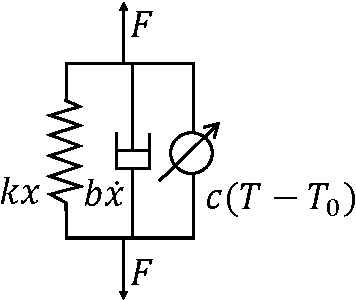
\includegraphics[width=\textwidth]{Model_muscle-cropped_compatible.pdf}
		%\centering\includegraphics[width=\textwidth]{example-image-a}
		\caption{\label{ModelMus}}
	\end{subfigure}
	\begin{subfigure}[t]{0.31\textwidth}
		\centering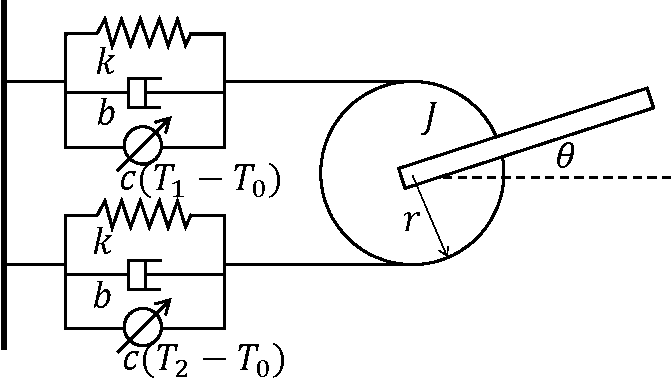
\includegraphics[width=\textwidth]{Model_anta-cropped_compatible.pdf}
		%\centering\includegraphics[width=\textwidth]{example-image-a}
		\caption{\label{ModelAnt}}
	\end{subfigure}
	\begin{subfigure}[t]{0.22\textwidth}
		\centering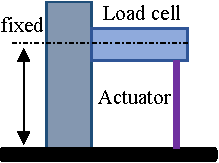
\includegraphics[width=\textwidth]{modeling_static_v2-cropped_compatible.pdf}
		%\centering\includegraphics[width=\textwidth]{example-image-a}
		\caption{\label{static_sch}}
	\end{subfigure}
	\begin{subfigure}[t]{0.22\textwidth}
		\centering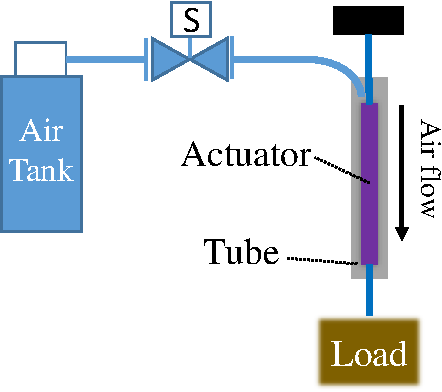
\includegraphics[width=\textwidth]{Static2(v2)_v4-cropped_compatible.pdf} % An old name of dynamic experiment : static2_v2
		%\centering\includegraphics[width=\textwidth]{example-image-a}
		\caption{\label{dynamic_sch}}
	\end{subfigure}
	\caption[Modeling of the \scps]{\subref{ModelMus} The \scps can be expressed as a combination of a spring, damper, and temperature-dependent system. \subref{ModelAnt} The \anta can be expressed with two complimentary muscles, which change the angular position. \subref{static_sch} Scheme of the static experiment. \subref{dynamic_sch} Scheme of the dynamic experiment.}
	\label{model+exp_sch}
\end{figure}

\subsection{Static Experiment}
The aim of the static experiment was to verify equation \eqref{thermo-mechanical_model} and achieve first and second aims mentioned in section \ref{section_aimsappa}. In other words, correlation of the \scpnospace's length and the tension was investigated at various temperatures. 

It can be said that muscles have a length $l_{0}$ at ambient temperature with \SI{0}{\newton} tension. Taking $l_{0}$ as standard, experiments were conducted by changing length \SI{15}{\milli\meter} gradually. Also, five kinds of voltage were used - \SI{0}{\volt}, \SI{1.0}{\volt}, \SI{1.8}{\volt}, \SI{2.2}{\volt}, and \SI{2.6}{\volt}. 
Following processes were carried out.

\begin{enumerate}
\item Initial length of the \scp was adjusted to $l_0$.
\item We started to apply a constant voltage to the muscle and waited until the muscle's length and temperature became steady.
\item When the muscle became steady, we started recording its physical properties, such as length, tension, temperature, and time.
\item We gradually increased the length of muscle to $l_0+d$.
\item We gradually decreased the length of muscle to $l_0$.
\item End of recording. After cooling to ambient temperature, we repeated 1-5 at other voltages.
\end{enumerate}

Results of the static experiment were shown in figure \ref{static1_results}. Each of the temperature indicated in legend corresponded to $T_{steady}$. In figure \ref{static1_result}, we could observe slight hysteresis. This characteristic graph can be linearly regressed as figure \ref{static1_line}. Also, by obtaining force at 10\% strain for each temperature, we could check that the force was linearly proportional to $T_{steady}$. (Figure \ref{static1_dot}) By analyzing the graph in figure \ref{static1_result}, we acquired the values of $k$, $c$ in \eqref{thermo-mechanical_model}.
\begin{equation}
k=\SI{304}{\newton\per\meter}, c=\SI{0.0501}{\newton\per\degreeCelsius}. \notag
\end{equation}

\begin{figure}[t]
	\centering
	\begin{subfigure}[t]{0.32\textwidth}
		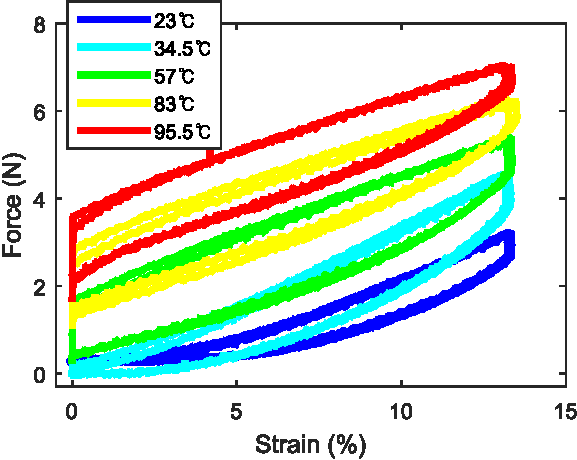
\includegraphics[width=\textwidth]{ForceStrain-cropped.pdf}
		\caption{\label{static1_result}}
	\end{subfigure}
	~
	\begin{subfigure}[t]{0.32\textwidth}
		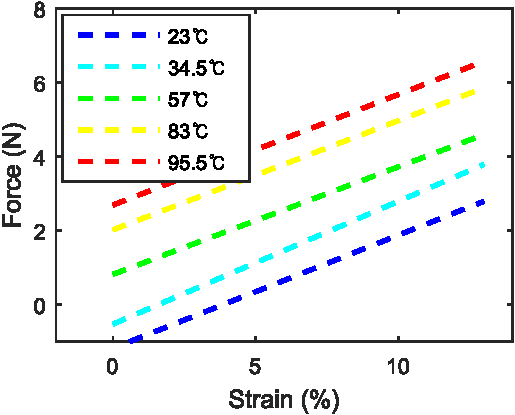
\includegraphics[width=\textwidth]{ForceStrain_line-cropped.pdf}
		\caption{\label{static1_line}}
	\end{subfigure}
	~
	\begin{subfigure}[t]{0.32\textwidth}
		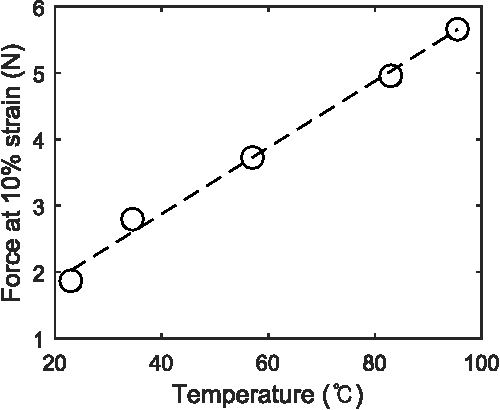
\includegraphics[width=\textwidth]{ForceStrain_dot-cropped.pdf}
		\caption{\label{static1_dot}}
	\end{subfigure}
	\caption[Results of the static experiment]{\subref{static1_result} Characteristic curves of \scp for various $T_{steady}$. \subref{static1_line} Linear graph of correlation between tension(force) and strain. \subref{static1_dot} Tension is linearly proportional to $T_{steady}$.}
	\label{static1_results}
\end{figure}

\subsection{Dynamic Experiment}\label{section_dynamic} % Important!!
The aim of the dynamic experiment was to achieve the third to the fifth aims as mentioned in section \ref{section_aimsappa}.
As introduced in section \ref{section_electrical_control}, forced air flow was periodically stopped and resumed to control the thermal conductivity of the \scpnospace.
This mechanism was performed by opening the solenoid valve in a constant ratio at each period. For example, if we make the valve be opened for \SI{70}{\milli\second} and closed for the next \SI{30}{\milli\second}, the ratio is 70\% in this situation. 
%From now on, we will call this `cooling ratio' and use variable name $r$.
The ratio will be referred as `cooling ratio' and variable name $r$ will be used from henceforth.
 
%With simple assumption, we can simply guess that $\lambda$ will be proportional to $r$, as equation \eqref{dynamic_simple_model}.
%\begin{equation} \label{dynamic_simple_model}
%\lambda = \lambda_{N}+(\lambda_{F}-\lambda_{N})\cdot r (0\leq r \leq 1)
%\end{equation}
%But, the air flow will keep for a short time right after the valve is closed. Therefore, it is expected that thermal conductivity will be constant if ratio is bigger than $r_{c}$. So, we can modify \eqref{dynamic_simple_model} into \eqref{dynamic_complicated}. 
%
%\begin{equation} \label{dynamic_complicated}
%\lambda = \begin{cases}
%\lambda_{N}+(\lambda_{F}-\lambda_{N})\cdot (r/r_{c}) & r_{c1}<r<r_{c2} \\
%\lambda_{F} & r>r_{c2} \\
%\end{cases}
%\end{equation}

The period of opening and closing was \SI{100}{\milli\second}, which was carefully chosen to achieve the best performance. If the period is too long, the thermal conductivity of the \scps will periodically change. On the other hand, if the period is too short, the solenoid valve won't perform well because it will take minimal time to open the valve. 

For the dynamic experiment, we carried out the following processes. We used constant voltage - \SI{2.59}{\volt}. Cooling ratio was variously changed, including $0$(Natural cooling, $\lambda_{N}$), and $1$(Complete forced cooling, $\lambda_{F}$). Also, five compressed air cans were implemented alternatively in order to maintain constant air pressure. 
\begin{enumerate}
\item When the muscle became $T=T_{ambient}$, we started recording time and temperature.
\item Constant power was applied until it reached the steady state.
\item After reaching $T=T_{steady}$, the power was disconnected and the cooling was started. 
\item When the muscle's temperature reached $T=T_{ambient}$ again, we stopped recording. 
\item We repeated the process 1-4 with other voltages and cooling ratios.
\end{enumerate}


\begin{figure}[t]
	\centering
	\begin{subfigure}[t]{0.45\linewidth}
		\centering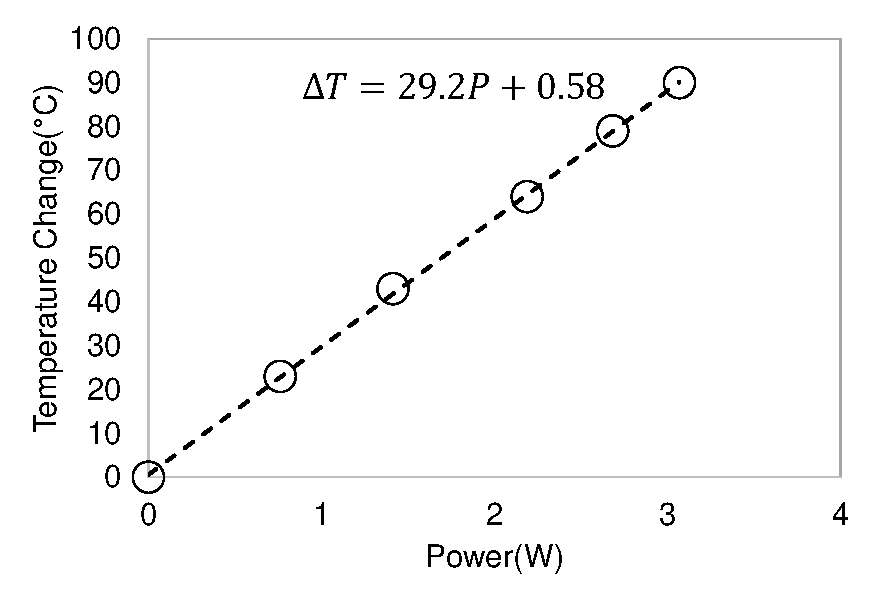
\includegraphics[width=\textwidth]{powerdeltaT-graph_v5.pdf}
		\caption{\label{powerdeltaT}}
	\end{subfigure}%
	\begin{subfigure}[t]{0.45\linewidth}
		\centering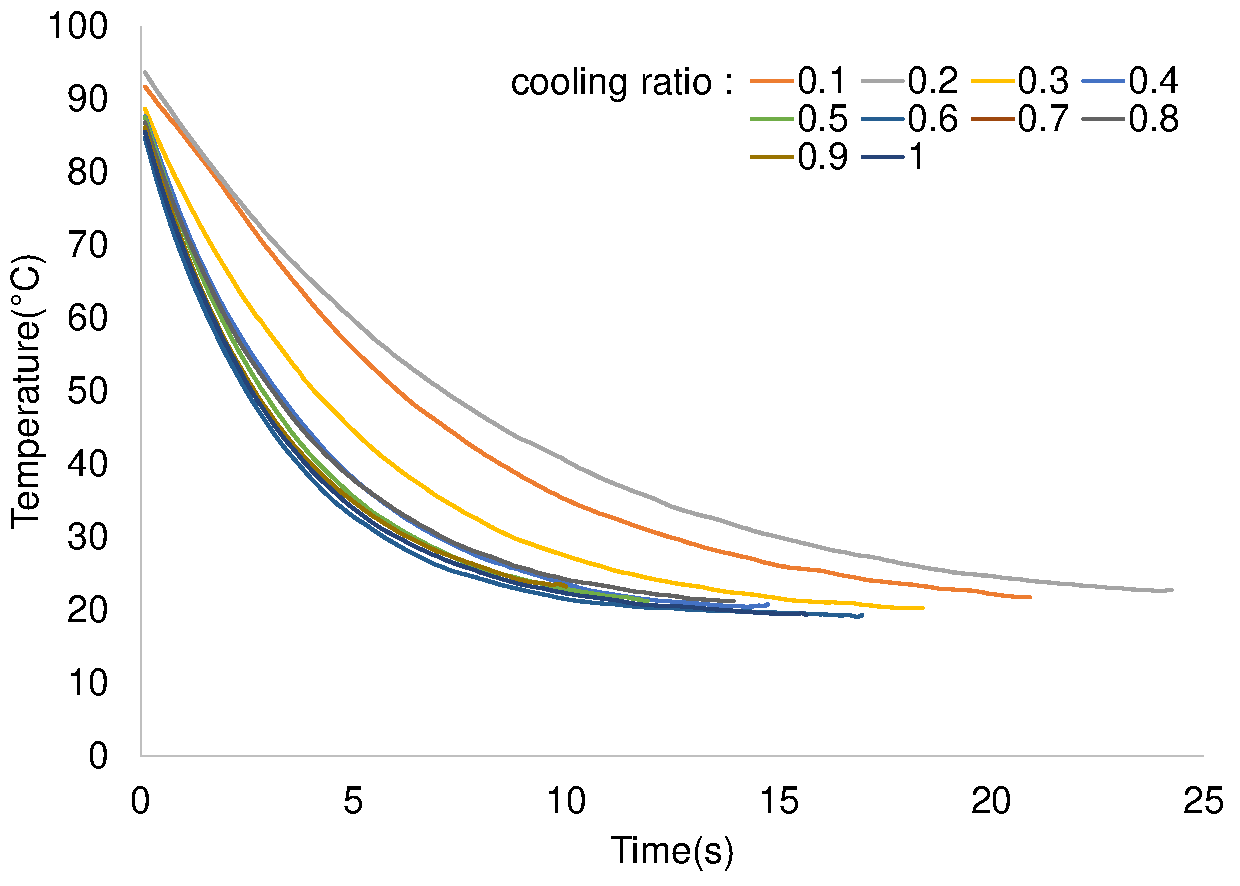
\includegraphics[width=\textwidth]{coolinggraph_v5.pdf}
		\caption{\label{coolinggraph}}
	\end{subfigure}
	\caption[Results of the dynamic experiment]{\subref{powerdeltaT} Temperature changes proportionally to power. \subref{coolinggraph} After power was shut down and forced cooling had began, temperature decreased exponentially.}
	\label{result_dynamic}
\end{figure}
%Based on experimental data, we calculated muscle's specific heat $C_{th}$ and thermal conductivity $\lambda$. In detail, we checked that $P$, $\Delta{T}$, $C_{th}$, $\lambda$, and time constant of temperature change $\tau$ satisfies equation \eqref{dynamic_calculation_power} and \eqref{dynamic_calculation_tau}. 

First, by graphing the relation between power $P$ and temperature shift $\Delta{T}=T_{steady}-T_{ambient}$, we could check that they were linearly proportional as \eqref{dynamic_calculation_power}.
Also, we could find the fact that the temperature of \scp changes exponentially as shown in figure \ref{coolinggraph}. This was in line with  \eqref{thermo-electrical_model}.

\begin{equation} \label{dynamic_calculation_power}
P = \lambda\Delta{T}
\end{equation}
By applying \eqref{dynamic_calculation_power} to a heating graph, we could get $\lambda_{N}$ according to figure \ref{powerdeltaT}. Then, while calculating the time constant of the heating graph, we could calculate \scp system's specific heat $C_{th}$ with \eqref{dynamic_calculation_tau}.\footnote{This was measured three times, resulting \SI{51.3}{\second}, \SI{54.1}{\second}, and \SI{53.0}{\second}. The average value was \SI{52.8}{\second}.} 

\begin{equation}
\lambda_{N}=\SI{3.42e-2}{\watt\per\degreeCelsius}, C_{th}=\SI{1.81}{\joule\per\degreeCelsius}. \notag
\end{equation}
Now, we have the value of $C_{th}$, so the thermal conductivity can be obtained by using \eqref{dynamic_calculation_tau}. Analysis for each cooling graph is shown in figure \ref{analysis_dynamic}.

\begin{equation} \label{dynamic_calculation_tau}
\lambda = \frac{C_{th}}{\tau}
\end{equation}

\begin{figure}[t]
	\begin{subfigure}[t]{0.52\linewidth}
		\centering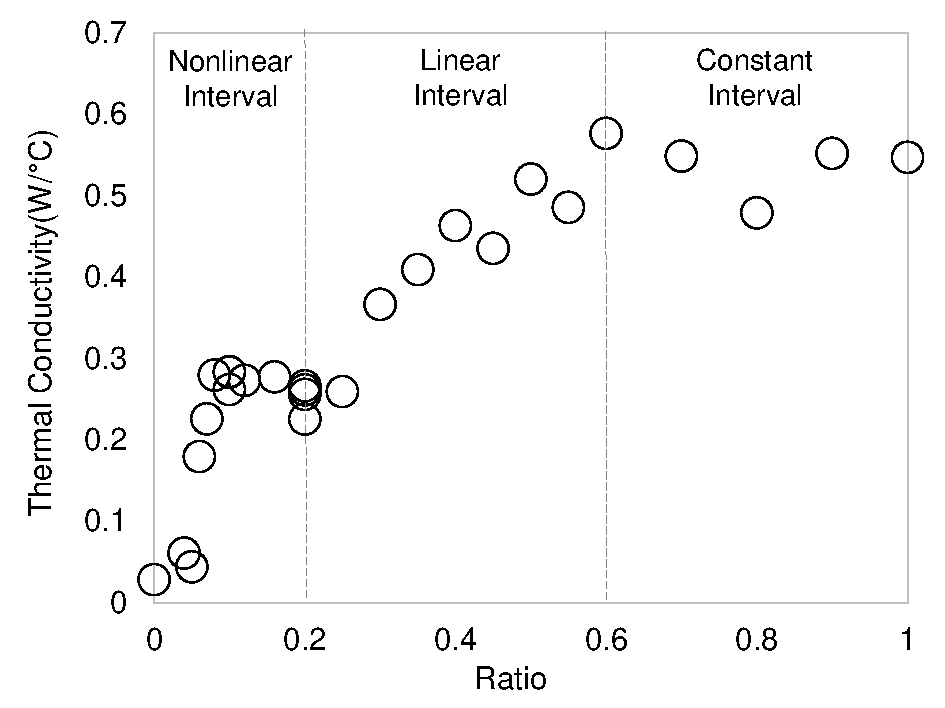
\includegraphics[width=\textwidth]{intervals_v3.pdf}
		\caption{\label{dynamic_proportional}}
	\end{subfigure}%
	\begin{subfigure}[t]{0.39\linewidth}
		%TODO : error - svg file not found...ㅠㅠ
		%\centering\includesvg[width=\textwidth]{../images/example}
		\centering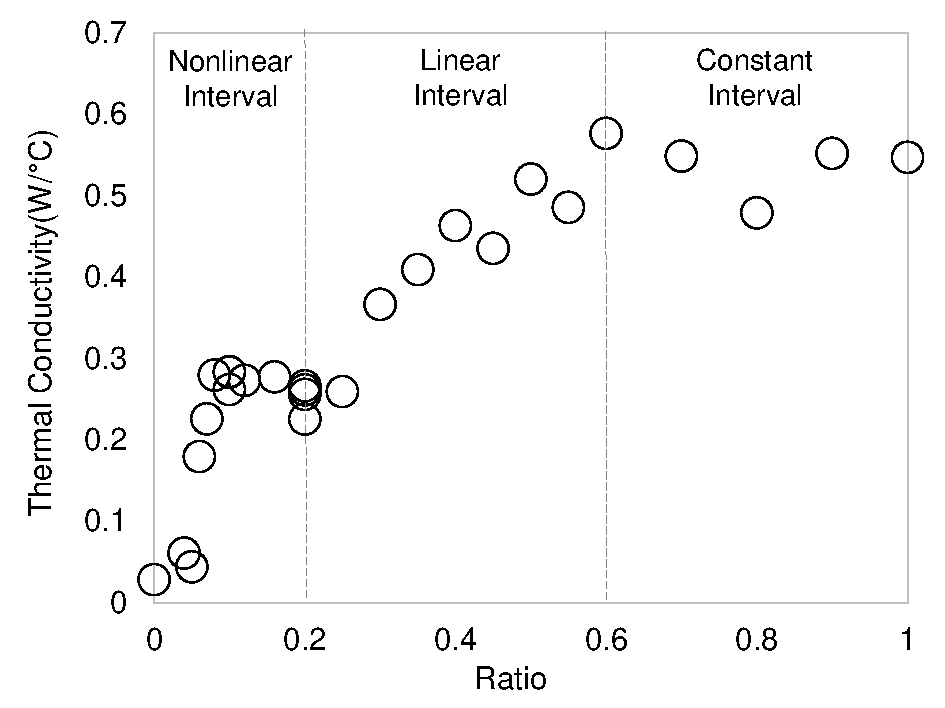
\includegraphics[width=\textwidth]{intervals_v3.pdf}
		\caption{\label{linear_interval}}
	\end{subfigure}
	\caption[Analysis of the dynamic experiment]{\subref{dynamic_proportional} $\lambda$ was linearly proportional to cooling ratio $r$ when $0.2<r<0.6$.  \subref{linear_interval} $\lambda$ could be calculated with the equation \eqref{lambda_control}.}
	\label{analysis_dynamic}
\end{figure}

In figure \ref{dynamic_proportional}, we can observe that the thermal conductivity in function of $r$ can be divided into three parts - nonlinear, linear, and constant interval. If $r<0.2$, $\lambda$ rapidly increased near $r=0.1$. Also, $\lambda$ wasn't increased anymore if $r>0.6$, {\it i.e.} $\lambda = \lambda_{F}$. This can be also observed from the cooling graph in figure \ref{coolinggraph}.
Therefore, the linear interval was chosen for the \Apcnospace.(Figure \ref{linear_interval}) The thermal conductivity in controllable(linear) interval was usually higher than cooling by computer fans, which were used by Yip \etalspace \cite{yip} and determined to be $\lambda_{fan}=\SI{0.30}{\watt\per\degreeCelsius}$.
\footnote{
	Meanwhile, we had to check that the load used in the dynamic experiment didn't affect muscle's thermal power. 
	Total electrical power of muscle was about $(\SI{1.0}{\volt})^2/(\SI{2.5}{\ohm})=\SI{0.4}{\watt}$, and cooling speed was about $\SI{1.39}{\joule\per\degreeCelsius} \cdot \SI{1}{\degreeCelsius\per\second}=\SI{1.39}{\watt}$ while gravitational power was about  $\SI{0.4}{\kilo\gram} \cdot  \SI{9.8}{\meter\per\second\square} \cdot \SI{0.001}{\meter\per\second}=\SI{0.004}{\watt}$. So we concluded that the load didn't affect the measurement of muscle's thermal properties.
}

\begin{equation} \label{lambda_control}
\lambda = 0.77\cdot r + 0.10 (\si{\watt\per\degreeCelsius}), 0.2\leq r \leq 0.6.
\end{equation}


%Meanwhile, we have to justify the approximation used in section \ref{section_dynamic_appa}. 



